\documentclass[12pt, oneside]{article}
\usepackage{graphicx}
\usepackage{setspace,amssymb,latexsym,amsmath,amscd,epsfig,amsthm,wasysym}
\usepackage{multirow}
\usepackage[nohead, margin=0.5in]{geometry}
\usepackage{enumitem}
\usepackage{subcaption}
\usepackage[titletoc]{appendix}
%\geometry{left=0.5in,right=0.5in,top=0.3in,bottom=0.5in} 

\usepackage{tikz}
\usetikzlibrary {positioning}
\usetikzlibrary{arrows.meta}
\usetikzlibrary{math} %needed tikz library
\usepackage{pgfplots}
\pgfplotsset{compat=1.11}
\usetikzlibrary{datavisualization}
\pagestyle{empty}

% hyperlink stuff
\usepackage{hyperref}
\hypersetup{
  colorlinks = true,
  linkcolor = black,
  urlcolor = black
}
\urlstyle{same}

% Some macros
\newcommand{\ket}[1]{\vert{#1}\rangle}
\newcommand{\bra}[1]{\langle{#1}\vert}
\newcommand{\braket}[2]{\langle{#1}\vert{#2}\rangle}
\newcommand{\matelm}[3]{\langle{#1}\vert{#2}\vert{#3}\rangle}
\newcommand{\subscript}[1]{\ensuremath{_{\textrm{#1}}}}
\newcommand{\superscript}[1]{\ensuremath{^{\textrm{#1}}}}
\newcommand{\sumation}[3]{\underset{#1}{\overset{#2}{\sum}}#3}
\newcommand{\fullsum}[3]{\underset{#1=#2}{\overset{#3}{\sum}}}
\newcommand{\expectation}[1]{\langle{#1}\rangle}

\title{Notes On Star Removal In Stereo HI Data}
\begin{document}
  \maketitle
  \newpage
  \tableofcontents
  \newpage
  
  \section{Introduction}
    The conditioning of STEREO HI L2 data for use in IPS tomography requires multiple steps. The processing chain first requires the extraction of pixel information from the L2 data files. This is primarily done using software provided by the SolarSoftWare (SSW) IDL libraries. Once the data is extracted, the next step is to remove stars, and enhance Thomson scattered light. The final link in the processing chain is the binning and formatting of the data (into points files) for the input into the IPS tomography.

    %\afge$
  
  \section{Data Extraction}
    The initial extraction of data (brightness) is done using the SSW IDL libraries. STEREO HI, L2, 11 day background subtracted, DNS images are downloaded from \url{https://www.ukssdc.ac.uk/solar/stereo/data.html}, and the data is extracted. At the same time the data is extracted, the SSW IDL libraries are used to remove background light, and reduce light from stars. In addition to background light removal the SSW IDL libraries are used to determine the right ascension and declination of each pixel. %Further discussion of the SSW IDL routines used in this process can be found in appendix \ref{appendix_ssw}
    
  \section{Star Mitigation}
    %The brightness of Thomson scattered light is very small relative to the background stars. Thus, it is important to remove all light due to stars. For the purposes of star removal, the stars are considered as outliers to the local pixel data. This assumption reduces the process of removing stars to looking for outliers in the brightness data. 
\subsection{Outlier Identification and Removal}
In order to identify outliers the image data (that is of resolution $res \times res$) is first processed by the SSW libraries. The image is then divided into a grid with dimension $n \times n$. The cells in this grid constitute a dataset 
\begin{equation}
  D = \{X_1, X_2,\dots,X_{n^2}\}
\end{equation}
$n$ can be computed using the dimensions of each cell $\left(m\right)$
\begin{equation}
  n = int\left( \frac{res}{m} \right) + H\left(res\ mod\ m \right)
\end{equation}
Where $H(x)$ is the Heaviside step function. Each of the cells is then scanned for outlier data points.

In order to identify outliers, robust statistical analysis is used. The median $\left(\overset{\sim}{X}_i\right)$ value of each cell's dataset $\left(X_i\right)$ is then calculated, and used as a representation of the central value of $X_i$. To determine the spread of data in each cell, the \textbf{median absolute deviation from the median $\left(\hat{\sigma}\right)$} is used.  The range of acceptable values from $X_i$ are determined by the following
\begin{equation}
  \overset{\sim}{X_i} - k \hat{\sigma} < x_{ij} < \overset{\sim}{X_i} + k \hat{\sigma}
  \label{eqn:accept_range}
\end{equation}
Where $x_{ij}$ is the $j^{th}$ pixel from $X_i$, and $k$ is a parameter used to control the spread of the acceptable range of data. Values that fall outside the range in Inequality \ref{eqn:accept_range} are replaced by $\overset{\sim}{X_i}$. \textbf{Note:} One possible improvement, could be to replace outliers with the mean value of the data in the immediate surroundings of the outlier. The values currently being used for the above parameters, for camera one can be found in Table \ref{tbl_outlier_id_params}.

\begin{table}[h]
  \center
  \begin{tabular}{|c|c|c|l|}
    \hline 
    \rule[-1ex]{0pt}{2.5ex} Parameter & Cam 1 & Cam 2 & Description \\ 
    \hline  
    \rule[-1ex]{0pt}{2.5ex} $res$ & $1024$ & $1024$ & resolution of image \\
    \hline 
    \rule[-1ex]{0pt}{2.5ex} $m$ & $50$ & $50$ & dimensions of each cell \\ 
    \hline 
    \rule[-1ex]{0pt}{2.5ex} $k$ & $3.0$ & $3.0$ & parameter for controlling spread of data in each cell \\ 
    \hline 
  \end{tabular}
  \caption{The values currently being used for each parameter, for camera one and camera two.}
  \label{tbl_outlier_id_params}
\end{table}  

\subsection{Median Absolute Deviation of the Median}
The \textbf{median absolute deviation from the median $\left(\hat{\sigma}\right)$} is a way of determining the spread of a dataset from its central value. For this analysis the central value will be represented by the median $\left(\overset{\sim}{X}\right)$. The median absolute deviation from the median is a robust statistical method that is resistant to the effects of outlier data points. In this work the $\hat{\sigma}$ is used as a replacement for the standard deviation $\left(\sigma\right)$ of a dataset.

Given a dataset $X = \{x_1, x_2,\dots,x_{m^2}\}$, the median is first calculated 
\begin{equation}
  \overset{\sim}{X} = median(X)
  \label{eqn:median}
\end{equation}
Once the median has been determined the $\hat{\sigma}$ can be calculated for $X$
\begin{equation}
  \hat{\sigma} = median \left( | x_i - \overset{\sim}{X} | \right),\ for\ i=1,2,\dots,m^2
\end{equation}
Now $\hat{\sigma}$ and $\overset{\sim}{X}$ are used in the same manner as the standard deviation and mean to determine outliers. That is only values in the range from Inequality \ref{eqn:accept_range} are accepted. Values outside the range in Inequality \ref{eqn:accept_range} are replaced by $\overset{\sim}{X}$.
%\subsection{Outlier Removal}
There is a need to condition (remove stars) from data obtained from the STEREO HI spacecrafts. For this purpose the stars are treated as outlier data points from the image data obtained from STEREO. A multi step process is used to identify and remove outlier data.

STEREO HI, L2, 11 day background subtracted, DNS image data is downloaded from \url{https://www.ukssdc.ac.uk/solar/stereo/data.html}, and a first pass of star removal is preformed. This first pass consists of processing the downloaded data using the solarsoftware (SSW) IDL libraries. The stars are removed using the IDL routine \verb|subtract_star_map|, which utilizes a star map database. The data is then converted to S10 units using the SSW libraries. The result of the \verb|subtract_star_map| routine is to mainly reduce the relative brightness of stars. However, it looks as thought there is also some reduction in the number of stars. Currently the star map data base covers the data range 03/09/2007 to 01/05/2010. It is not clear as to how this effects data from 2011 on.

After applying the SSW \verb|subtract_star_map| routine, and converting the data to S10 units, the data is further processed using a MAD filter. During this process the data is split into a grid (bins). Each bin is then scanned, and a median value along with a MAD is obtained. The range of acceptable data values for the bin are determined
\begin{equation}
  \overset{\sim}{X} - k \hat{\sigma} < X_i < \overset{\sim}{X} + k \hat{\sigma}
  \label{eqn:accept_range2}
\end{equation}
Where $k$ is a parameter used to control the spread of acceptable range of data. Values that fall outside the range in \ref{eqn:accept_range2} are replaced with the $\overset{\sim}{X}$ for the bin. \textbf{Note:} One possible improvement could be to replace outliers with a local mean of data around the outlier. This method seems to remove a large portion of the stars. However, the resolution is reduced. A value of $k = 0.5$ results in the removal and replacement of about $70\%$ of the data in each bin. This requires that the bin sizes be relatively small $\left(10 \times 10\right)$ to keep a reasonable resolution.

The following images have had their brightness adjusted using ImageJ to insure a fair comparison. All images use $-32$ for the minimum displayed value, and $190$ for the maximum displayed value.
%
\begin{figure}
  \centering
  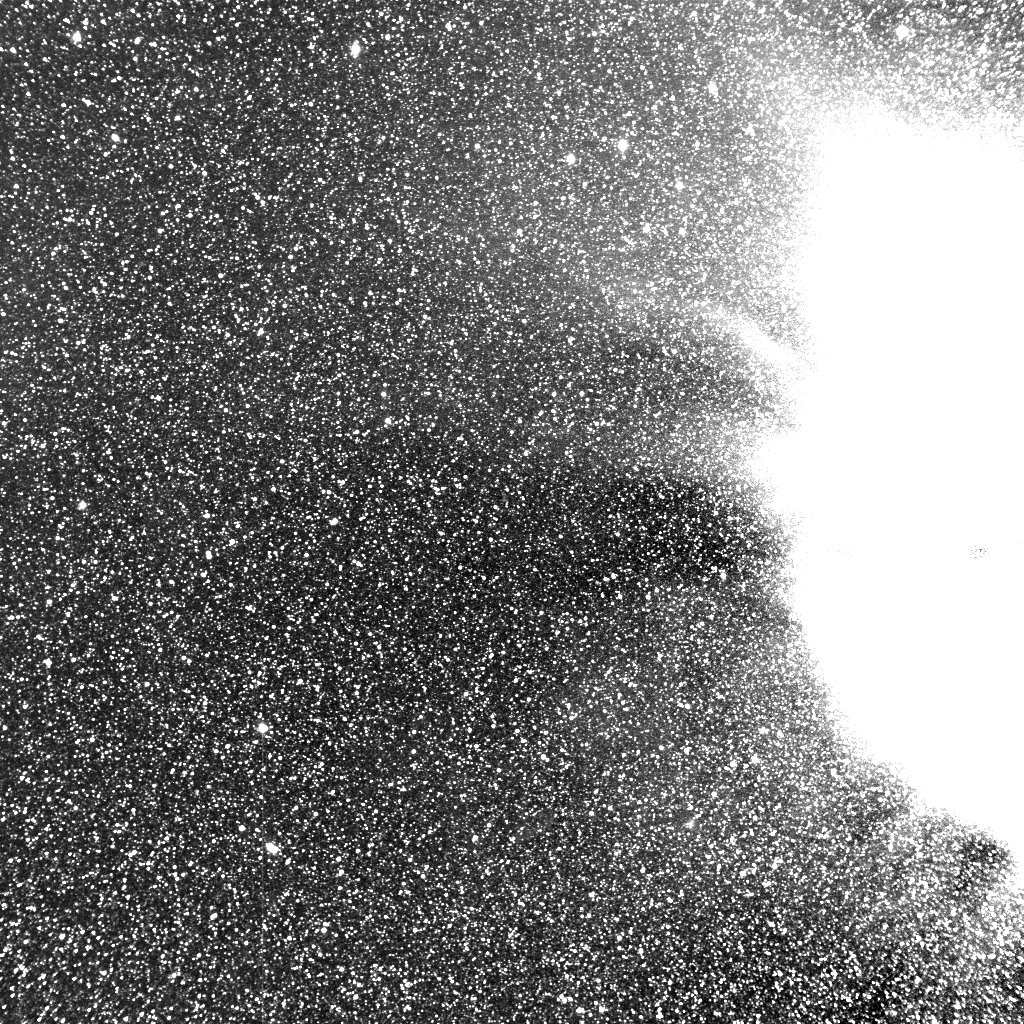
\includegraphics[scale=0.5]{../IMAGES/20110924_180901_24h1A_br11_WITH_STARS_S10_contrast_32_190.jpg} 
  \caption{STEREO HI-1A, 9/24/2011 18:09 UT, 11 day background subtraction, S10 units. Unprocessed.} 
  \label{fig:hi1a_with_stars_s10}
\end{figure}
%
\begin{figure}
  \centering
  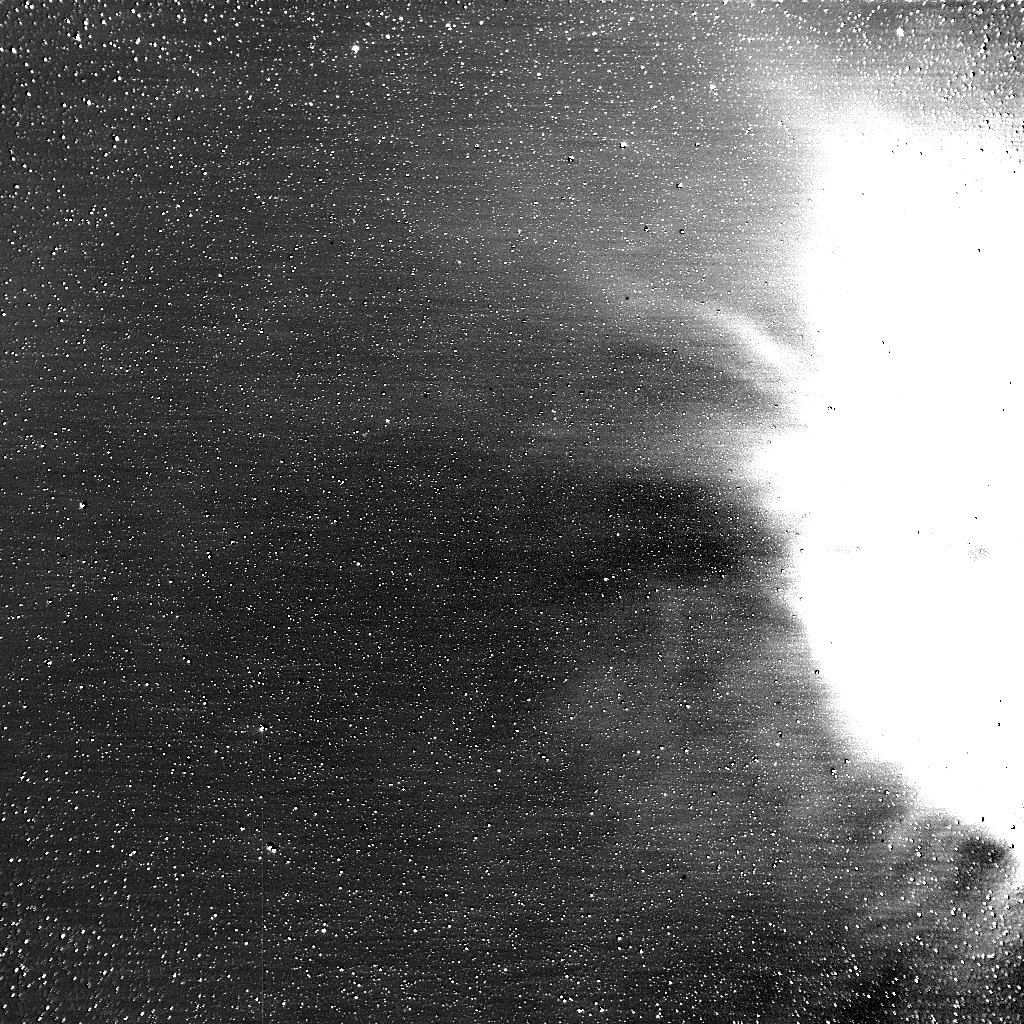
\includegraphics[scale=0.5]{../IMAGES/20110924_180901_24h1A_br11_NO_STARS_S10_contrast_32_190.jpg} 
  \caption{STEREO HI-1A, 9/24/2011, 18:09 UT, 11 day background subtraction, S10 units. Processed with subtract\_star\_map only.}
  \label{fig:hi1a_subtract_star_map}
\end{figure}
%
\begin{figure}
  \centering
  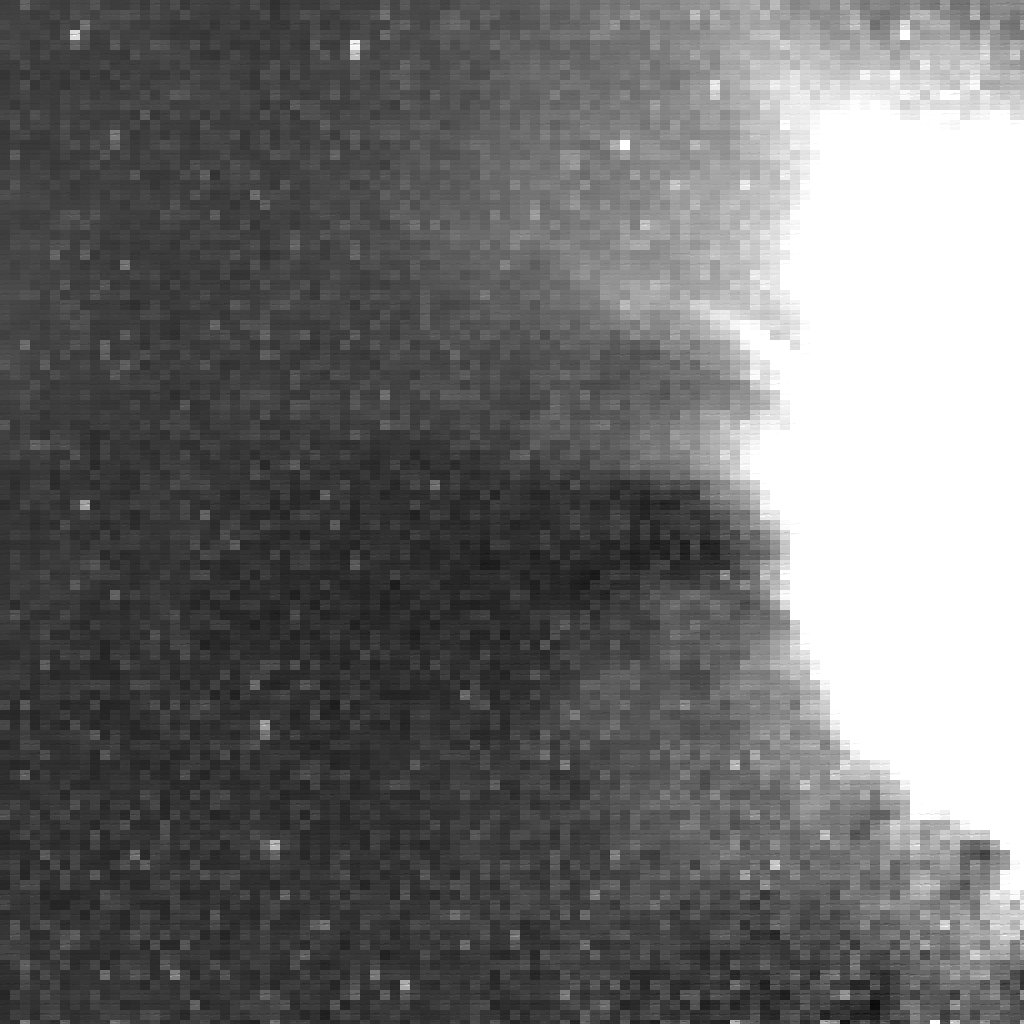
\includegraphics[scale=0.5]{../IMAGES/20110924_180901_24h1A_br11_WITH_STARS_0010_05stdev_contrast_32_190.jpg} 
  \caption{STEREO HI-1A, 9/24/2011, 18:09 UT, 11 day background subtraction, S10 units. Processed with outlier removal, with bin size $10 \times 10$, and $0.5 \hat{\sigma}$. No subtract\_star\_map routine applied.}
  \label{fig:fig:hi1a_0010bin_05stdev}
\end{figure}
%
\begin{figure}
  \centering
  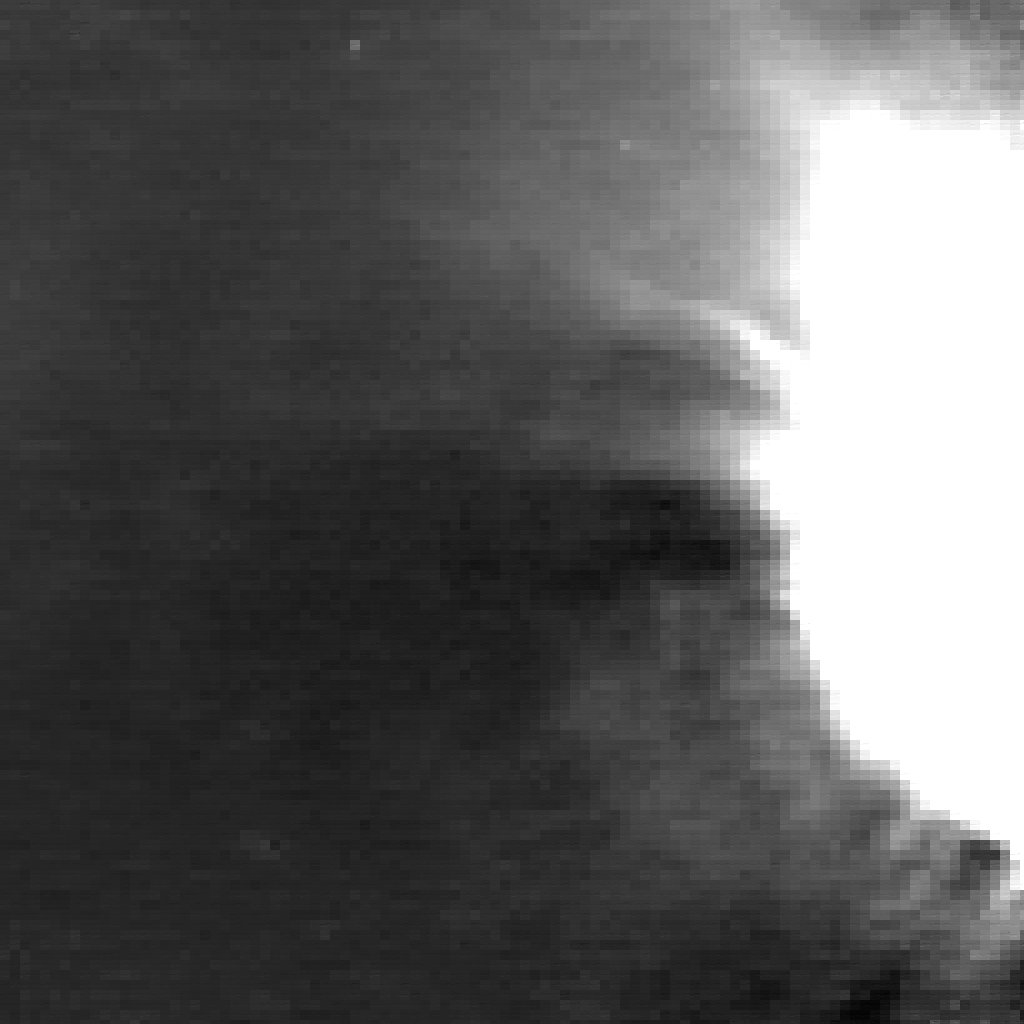
\includegraphics[scale=0.5]{../IMAGES/20110924_180901_24h1A_br11_NO_STARS_NO_STARS_0010_05stdev_contrast_32_190.jpg} 
  \caption{STEREO HI-1A, 9/24/2011, 18:09 UT, 11 day background subtraction, S10 units. Processed using subtract\_star\_map, and outlier removal with bin size $10 \times 10$, and $0.5 \hat{\sigma}$.}
  \label{fig:hi1a_subtract_star_map_0010bin_05stdev}
\end{figure}
%

























    
  \section{Data Binning}
    Once background light and stars have been removed the data is binned and formatted for input into the IPS tomography. The binning of the data consists of first splitting the data into a grid of $\ell \times \ell$ squares. After splitting the data into a grid, the mean of the brightness, right ascension, and declination is computed. It will be these mean values that will represent each bin. The values of $\ell$ will depend on how much of the sky each bin will cover. Table \ref{tbl_bin_dimensions} shows the dimensions of the bins currently in use for each camera.
\begin{table}[h]
  \center
  \begin{tabular}{|c|c|c|}
    \hline 
    \rule[-1ex]{0pt}{2.5ex} Device & $\ell$ & Degrees per bin  \\ 
    \hline 
    \rule[-1ex]{0pt}{2.5ex} Camera 1 & $51$ & $1 \times 1$  \\ 
    \hline 
    \rule[-1ex]{0pt}{2.5ex} Camera 2 & $14$  & $1 \times 1$ \\ 
    \hline 
  \end{tabular} 
  \caption{Dimensions for binning for each camera, and the resulting resolution.}
  \label{tbl_bin_dimensions}
\end{table}
  
  \section{Temporary}
    \subsection{Outlier Removal}
There is a need to condition (remove stars) from data obtained from the STEREO HI spacecrafts. For this purpose the stars are treated as outlier data points from the image data obtained from STEREO. A multi step process is used to identify and remove outlier data.

STEREO HI, L2, 11 day background subtracted, DNS image data is downloaded from \url{https://www.ukssdc.ac.uk/solar/stereo/data.html}, and a first pass of star removal is preformed. This first pass consists of processing the downloaded data using the solarsoftware (SSW) IDL libraries. The stars are removed using the IDL routine \verb|subtract_star_map|, which utilizes a star map database. The data is then converted to S10 units using the SSW libraries. The result of the \verb|subtract_star_map| routine is to mainly reduce the relative brightness of stars. However, it looks as thought there is also some reduction in the number of stars. Currently the star map data base covers the data range 03/09/2007 to 01/05/2010. It is not clear as to how this effects data from 2011 on.

After applying the SSW \verb|subtract_star_map| routine, and converting the data to S10 units, the data is further processed using a MAD filter. During this process the data is split into a grid (bins). Each bin is then scanned, and a median value along with a MAD is obtained. The range of acceptable data values for the bin are determined
\begin{equation}
  \overset{\sim}{X} - k \hat{\sigma} < X_i < \overset{\sim}{X} + k \hat{\sigma}
  \label{eqn:accept_range2}
\end{equation}
Where $k$ is a parameter used to control the spread of acceptable range of data. Values that fall outside the range in \ref{eqn:accept_range2} are replaced with the $\overset{\sim}{X}$ for the bin. \textbf{Note:} One possible improvement could be to replace outliers with a local mean of data around the outlier. This method seems to remove a large portion of the stars. However, the resolution is reduced. A value of $k = 0.5$ results in the removal and replacement of about $70\%$ of the data in each bin. This requires that the bin sizes be relatively small $\left(10 \times 10\right)$ to keep a reasonable resolution.

The following images have had their brightness adjusted using ImageJ to insure a fair comparison. All images use $-32$ for the minimum displayed value, and $190$ for the maximum displayed value.
%
\begin{figure}
  \centering
  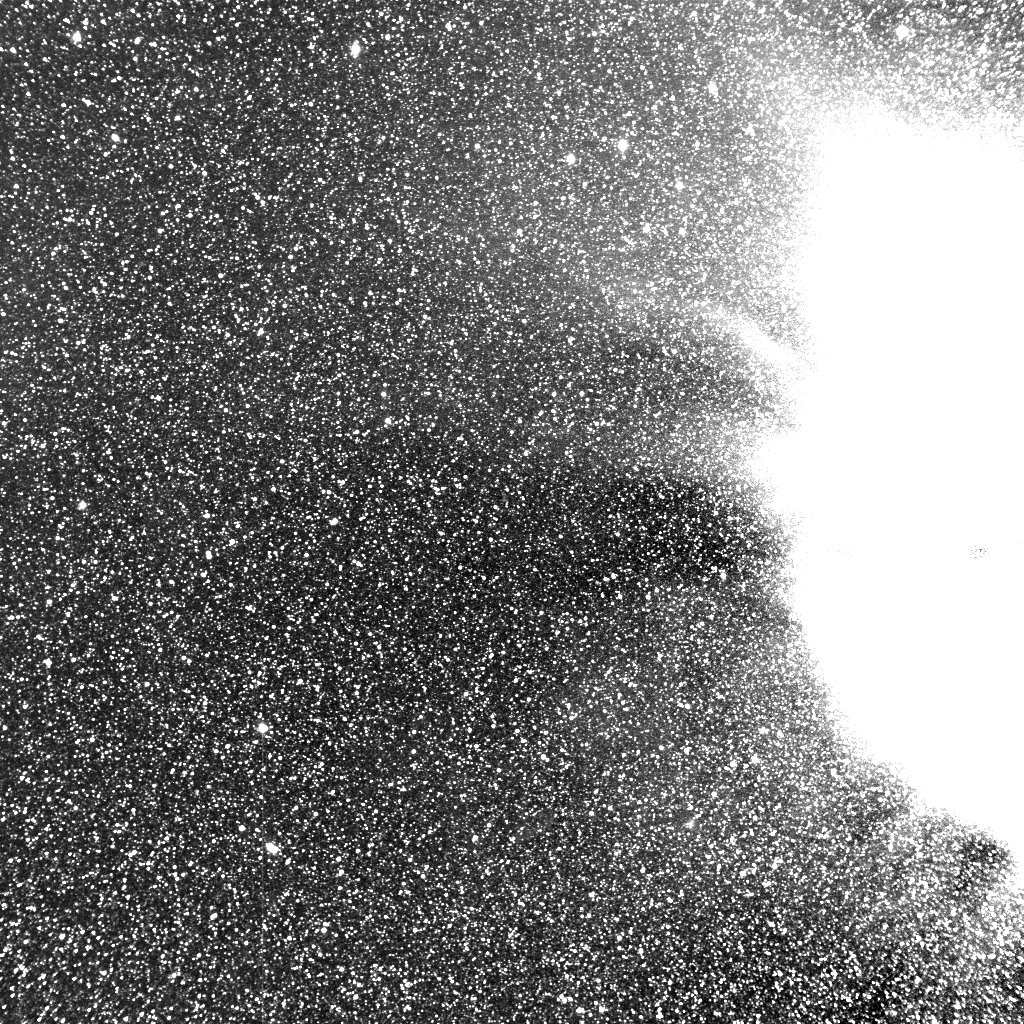
\includegraphics[scale=0.5]{../IMAGES/20110924_180901_24h1A_br11_WITH_STARS_S10_contrast_32_190.jpg} 
  \caption{STEREO HI-1A, 9/24/2011 18:09 UT, 11 day background subtraction, S10 units. Unprocessed.} 
  \label{fig:hi1a_with_stars_s10}
\end{figure}
%
\begin{figure}
  \centering
  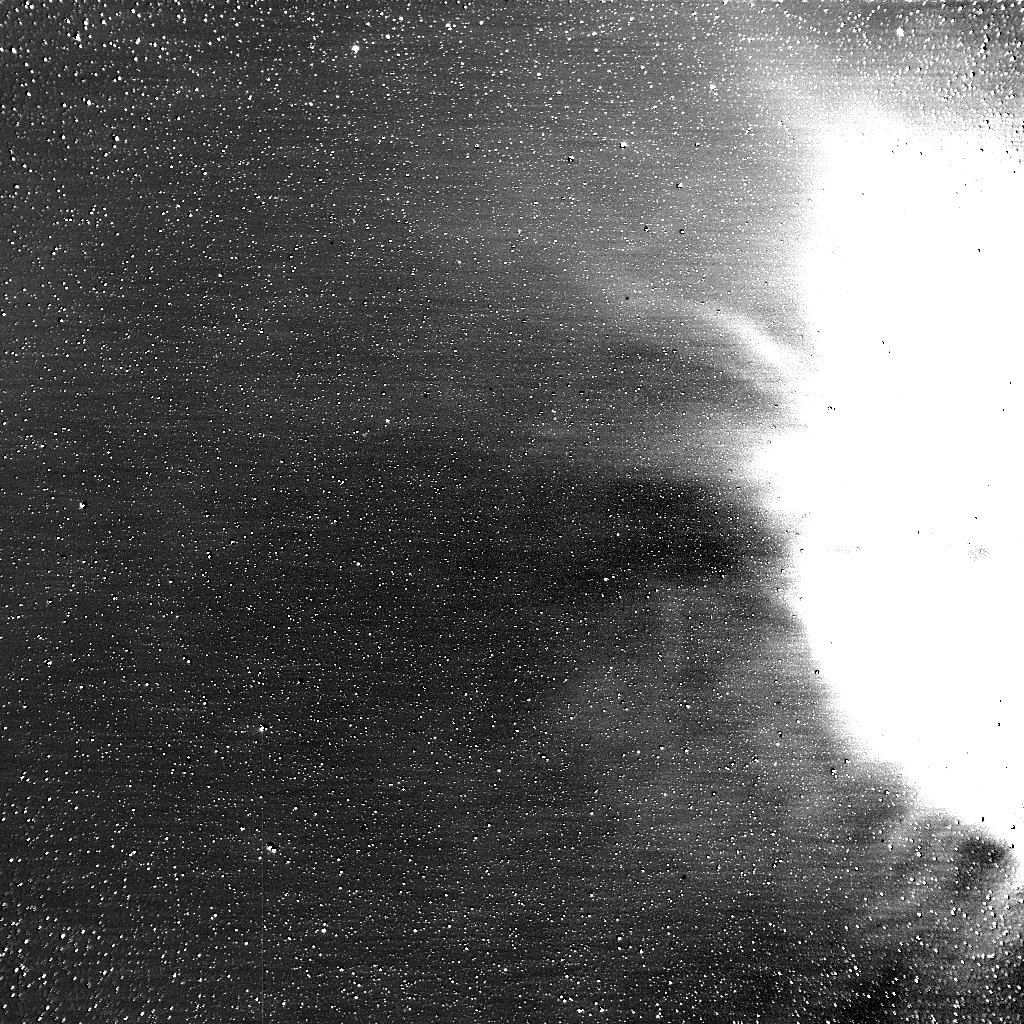
\includegraphics[scale=0.5]{../IMAGES/20110924_180901_24h1A_br11_NO_STARS_S10_contrast_32_190.jpg} 
  \caption{STEREO HI-1A, 9/24/2011, 18:09 UT, 11 day background subtraction, S10 units. Processed with subtract\_star\_map only.}
  \label{fig:hi1a_subtract_star_map}
\end{figure}
%
\begin{figure}
  \centering
  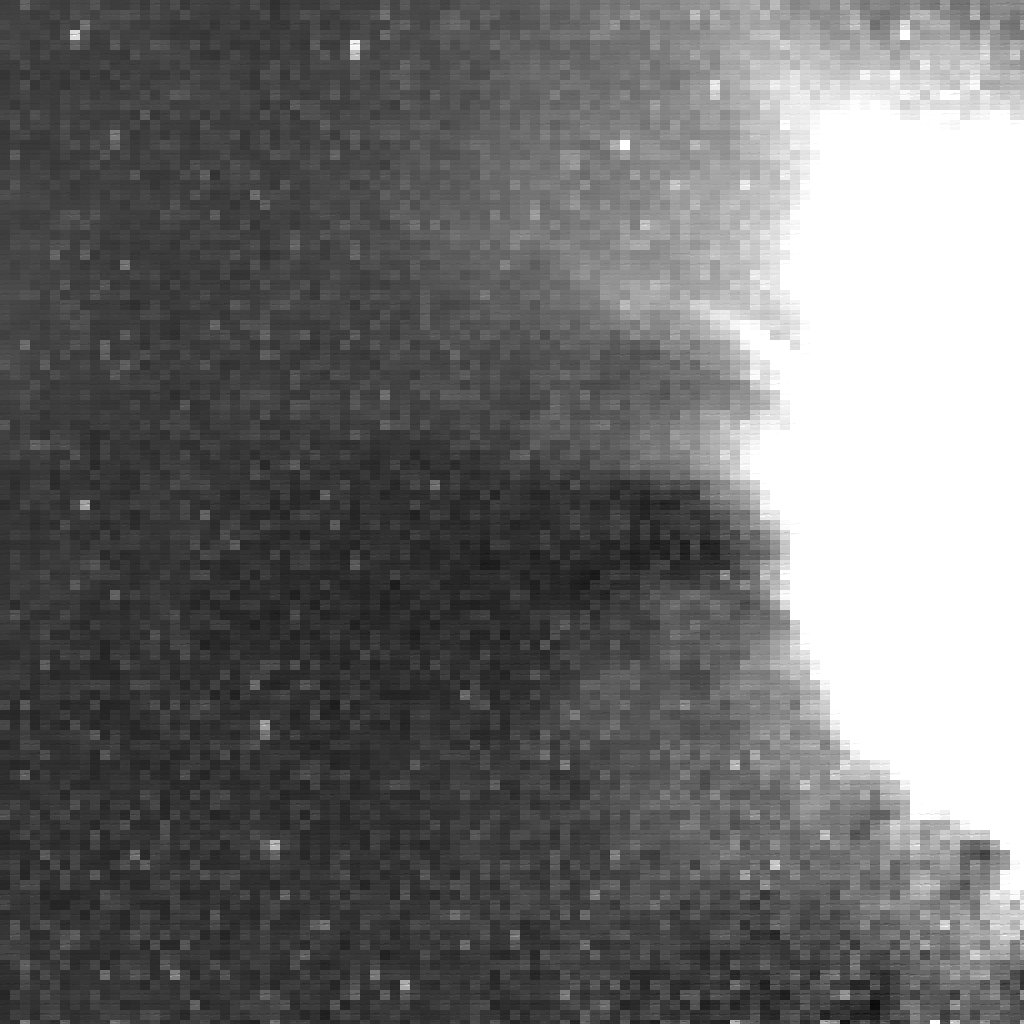
\includegraphics[scale=0.5]{../IMAGES/20110924_180901_24h1A_br11_WITH_STARS_0010_05stdev_contrast_32_190.jpg} 
  \caption{STEREO HI-1A, 9/24/2011, 18:09 UT, 11 day background subtraction, S10 units. Processed with outlier removal, with bin size $10 \times 10$, and $0.5 \hat{\sigma}$. No subtract\_star\_map routine applied.}
  \label{fig:fig:hi1a_0010bin_05stdev}
\end{figure}
%
\begin{figure}
  \centering
  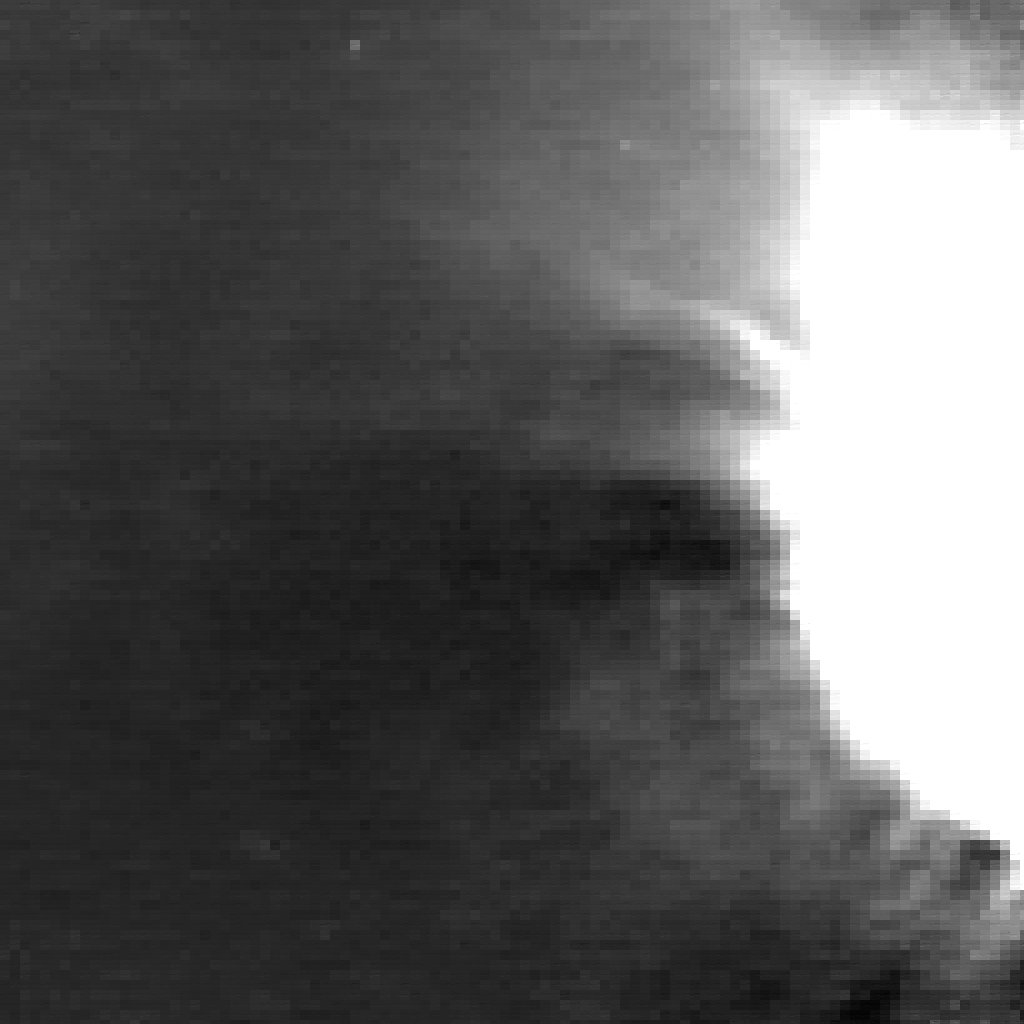
\includegraphics[scale=0.5]{../IMAGES/20110924_180901_24h1A_br11_NO_STARS_NO_STARS_0010_05stdev_contrast_32_190.jpg} 
  \caption{STEREO HI-1A, 9/24/2011, 18:09 UT, 11 day background subtraction, S10 units. Processed using subtract\_star\_map, and outlier removal with bin size $10 \times 10$, and $0.5 \hat{\sigma}$.}
  \label{fig:hi1a_subtract_star_map_0010bin_05stdev}
\end{figure}
%

























    
%  \begin{appendices}
%    \section{SolarSoftWare (SSW) IDL Library Routines}\label{appendix_ssw}
The SolarSoftWare (SSW) IDL library is used to extract downloaded data, and as a first pass to remove background light.
%    \section{Parameters and Comparisons}
blhal blhask bl bh blah
%  \end{appendices}
\end{document}





























